\subsection{CU16 Registrar Refacción}
Esta pantalla aparece cuando el administrador elige la opción de registrar una refacción desde la pantalla de 'Visualizar Refacciones, (figura\ref{fig:Pantalla Visualizar Refacciones Administrador - Vista de Escenarios}). En esta sección, el sistema solicita que el administrador ingrese la información para hacer el registro eb este caso es el Número de Inventario, para que Vehículo va destinado y por último una descripción de la refacción que se va a utilizar. En la parte inferior de la pantalla, tenemos dos botones con diferentes opciones:
\begin{itemize}
	\item \textbf{Registrar:} Al dar click en este botón, el sistema validará cada uno de los campos que han sido llenados, su formato y su contenido. En caso de que exista un error, el propio sistema mostrará un mensaje de error para que el administador corrija el error.
	\item \textbf{Cancelar:} El sistema regresa a la pantalla anterior \ref{fig:Pantalla Visualizar Refacciones Administrador - Vista de Escenarios} sin hacer algún registro.
\end{itemize} 
\begin{figure}[!h]
	\centering
	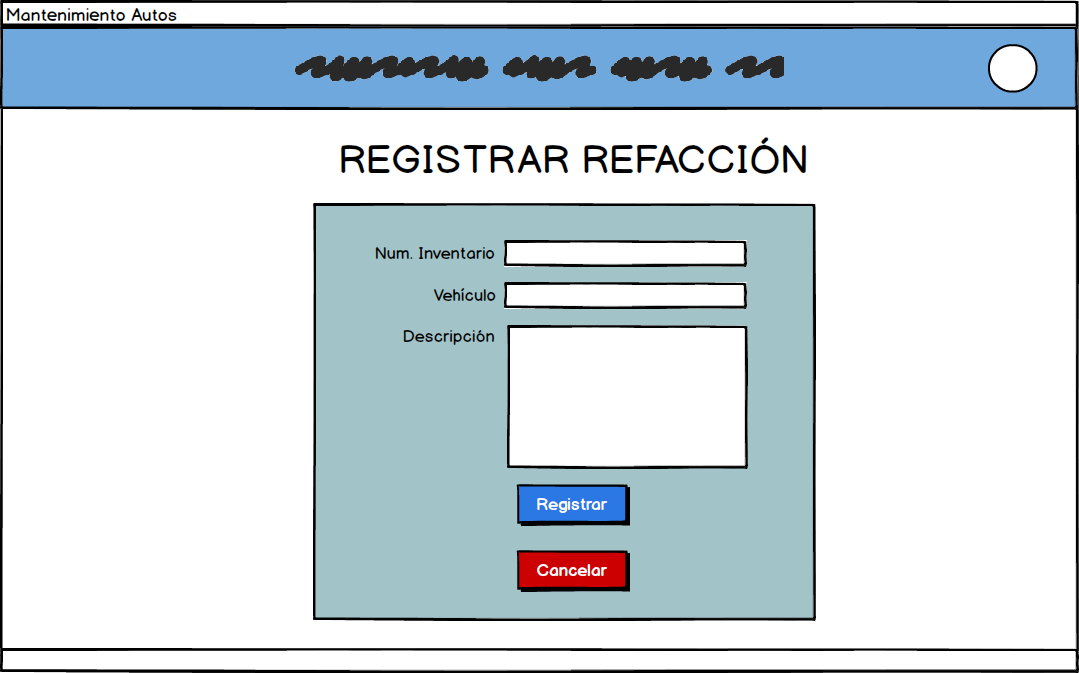
\includegraphics[width=0.8\textwidth]{./diseno/vescenarios/imagenes/registrarRefacciones}
	\caption{Pantalla Registrar Refacción - Vista de Escenarios}
	\label{fig:Pantalla Registrar Refacción - Vista de Escenarios}
\end{figure}
\begin{figure}[!h]
	\centering
	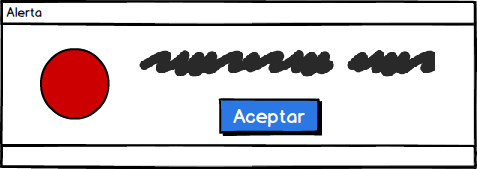
\includegraphics[width=0.3\textwidth]{./diseno/vescenarios/imagenes/alerta}
	\caption{Alerta Registro Refacciones- Vista de Escenarios}
	\label{fig:Alerta Registro Refacciones - Vista de Escenarios}
\end{figure}